\documentclass[ucs, notheorems, handout]{beamer}

\usetheme[numbers,totalnumbers,minimal,nologo]{Statmod}
\usefonttheme[onlymath]{serif}
\setbeamertemplate{navigation symbols}{}
\setbeamercolor{alerted text}{fg=blue}
\usepackage{physics}

\mode<handout> {
    \usepackage{pgfpages}
    %\setbeameroption{show notes}
    %\pgfpagesuselayout{2 on 1}[a4paper, border shrink=5mm]
    \setbeamercolor{note page}{bg=white}
    \setbeamercolor{note title}{bg=gray!10}
    \setbeamercolor{note date}{fg=gray!10}
}

\usepackage[utf8x]{inputenc}
\usepackage[T2A]{fontenc}
\usepackage[english, russian]{babel}
\usepackage{tikz}
\usepackage{ragged2e}
\usepackage{graphicx}
\usepackage{subfigure}


\usepackage{latexsym,amssymb}
\usepackage{amsmath}
\usepackage{amsfonts}
\usepackage{amsthm}

\DeclareMathOperator{\rk}{rk}
\DeclareMathOperator{\med}{med}
\DeclareMathOperator{\diag}{diag}
\DeclareMathOperator*{\argmin}{argmin}
\newcommand{\tX}[1]{\mathsf{#1}}
\newcommand{\iu}{\mathrm{i}\mkern1mu}

\title[Ошибки CSSA]
{Ошибки оценивания сигнала с помощью комплексного анализа сингулярного спектра}

\subtitle
{}

\author[Голяндина Н.Э., Сенов М.А.]
{Голяндина Нина Эдуардовна, \underline{Сенов Михаил Андреевич}
СПбГУ, кафедра статистического моделирования}

\institute[СПИСОК]{
Конференция СПИСОК-2022\\
Секция <<Вычислительная стохастика и статистические модели>>}

\date[Зачет]{Санкт-Петербург, 28 апреля 2022}

\begin{document}

\begin{frame}
  \titlepage
  \note{}
\end{frame}

\begin{frame}{Введение: Проблема}

$\tX{X} = (x_1, \ldots, x_{N})$ временной ряд длины $N$.\\
\vspace{1em}
\alert{Модель:} $\tX{X} = \tX{S} + \tX{R}$, $\tX{S}$ сигнал, $\tX{R}$ возмущение (шум или выброс).\\
\vspace{1em}
\alert{Задача:} Оценить сигнал $\tilde{\tX{S}} = F(\tX{X})$, $F$ --- используемый метод.\\
\vspace{1em}
\alert{Метод:} SSA (Singular Spectrum Analysis) [Golyandina et al., 2001] для вещественных рядов, CSSA (Complex Singular Spectrum Analysis) --- обобщение для комплексных рядов.\\
\vspace{1em}
\alert{Проблема:} Что лучше, с точки зрения величины ошибки $\tilde{\tX{S}} - \tX{S}$,

SSA$(\tX{X}_{\Re}) + \iu \text{SSA}(\tX{X}_{\Im})$ или CSSA$(\tX{X}_{\Re} + \iu \tX{X}_{\Im})$?

\end{frame}

\begin{frame}{Введение: Обозначения}
Рассмотрим временной ряд $\tX{X}=(x_1, \ldots, x_{N})$, $L$ длина окна, $K=N-L+1$.\\
\vspace{1em}
$\mathcal{M}_{r}$ --- пространство матриц размера $L \times K$ ранга не больше $r$.

$\mathcal{M}_{\mathcal{H}}$~--- пространство ганкелевых матриц $L\times K$.\\
\vspace{1em}
Оператор вложения $\mathcal{T}_L:\mathbb{R}^N \rightarrow \mathcal{M}_{\mathcal{H}}: \mathcal{T}_L (\tX{X}) = \mathbf{X} $,\\
$$\mathbf{X} = \begin{pmatrix}
           x_1 & x_2 & \ldots & x_{K}\\
           x_2 & x_3 & \ldots & x_{K+1}\\
           \vdots & \vdots & & \vdots\\
           x_{L} & x_{L+1} & \ldots & x_{N}
         \end{pmatrix}, K = N - L + 1,$$
$\mathbf{X}$~--- $L$-траекторная матрица $\tX{X}$.\\
\vspace{1em}
$\Pi_{r}:\mathcal{M}\rightarrow \mathcal{M}_r$,
$\Pi_{\mathcal{H}}:\mathcal{M} \rightarrow \mathcal{M}_{\mathcal{H}}$~--- проекторы на $\mathcal{M}_{r}$ и $\mathcal{M}_{\mathcal{H}}$ по норме Форбениуса.

    \note{}

\end{frame}

\begin{frame}{Введение: Ошибка восстановления}
Временной ряд $\tX{X}=(x_1, \ldots, x_{N})$, $L$ --- длина окна, $r$ --- ранг оцениваемого сигнала (ранга траекторной матрицы сигнала).
    \begin{block}{Алгоритм SSA (CSSA) выделения сигнала}
\begin{equation*}
	\tilde{\tX{S}} = \mathcal{T}^{-1}_{L} \Pi_{\mathcal{H}} \Pi_{r} \mathcal{T}_L (\tX{X}).
\end{equation*}
\end{block}

\alert{Модель:} $\tX{X} = \tX{S}(\delta)$, где $\tX{S}(\delta) = \tX{S} + \delta \tX{R}$ длины $N$ или \\ $\mathbf{H}(\delta) = \mathbf{H} + \delta \mathbf{E}$,
где $\mathbf{H}(\delta) = \mathcal{T}_L(\tX{S}(\delta))$, $\mathbf{H} = \mathcal{T}_L(\tX{S})$, $\delta\mathbf{E} = \mathcal{T}_L(\delta \tX{R})$.\\
\vspace{1em}
$\tilde{\tX{S}} = \mathcal{T}^{-1} \Pi_{\mathcal{H}} (\mathbf{H} + \delta\mathbf{H}^{(1)} + \delta^2\mathbf{H}^{(2)})$ из (Nekrutkin, 2008).\\
\vspace{1em}
$\tX{F} = \tilde{\tX{S}} - \tX{S} = \mathcal{T}^{-1} \Pi_{\mathcal{H}} (\delta\mathbf{H}^{(1)} + \delta^2\mathbf{H}^{(2)})$ ошибка восстановления.\\
\vspace{1em}
Рассматриваем $\delta = 1$,\\
\fbox{$\tX{F}^{(1)} = \mathcal{T}^{-1}_{L}(\mathbf{H}^{(1)})$ первый порядок ошибки восстановления.}

\end{frame}

\begin{frame}{Ошибка восстановления: Формула для $\mathbf{H}^{(1)}$}

Итак, рассматриваем $\delta = 1$, 
$\tX{X} = \tX{S}(1) = \tX{S} + \tX{R}$,

Тогда
$\tilde{\tX{S}} = \mathcal{T}^{-1} \Pi_{\mathcal{H}} (\mathbf{H} + \mathbf{H}^{(1)} + \mathbf{H}^{(2)}))$,

$\tX{F} = \tilde{\tX{S}} - \tX{S}$,

$\tX{F}^{(1)} = \mathcal{T}^{-1}_{L}(\mathbf{H}^{(1)})$.\\
\vspace{1em}
На основе результатов из (Константинов,~2018) и (Некруткин,~2010) была получена формула для $\mathbf{H}^{(1)}$ в случае достаточно маленького возмущения:

\begin{equation*} \label{eq:main}
	\mathbf{H}^{(1)} = \mathbf{P}^{\perp}_0 \mathbf{E} \mathbf{Q}_0 + \mathbf{P}_0 \mathbf{E},
\end{equation*}
где $\mathbf{P}_0$~--- проектор на пространство столбцов $\mathbf{H}$, \\$\mathbf{Q}_0$~--- проектор на пространство строк $\mathbf{H}$,\\ $\mathbf{P}^{\perp}_0 = \mathbf{I} - \mathbf{P}_0$, $\mathbf{I}$~--- единичная матрица.
\end{frame}

\begin{frame}{Ошибка восстановления: Теорема}
    CSSA-$\tX{F}^{(1)}$ первый порядок ошибки восстановления $\tX{S}$ с возмущением $\tX{R}$ метода CSSA,

    SSA-$\tX{F}^{(1)}_{\Re}$ первый порядок ошибки восстановления $\Re(\tX{S})$ с возмущением $\Re(\tX{R})$ метода SSA,

    SSA-$\tX{F}^{(1)}_{\Im}$ первый порядок ошибки восстановления $\Im(\tX{S})$ с возмущением $\Im(\tX{R})$ метода SSA.

    \begin{block}{Теорема \label{th:sum}}
        Пусть пространства столбцов траекторных матриц рядов $\tX{S}$, $\Re(\tX{S})$ и $\Im(\tX{S})$ совпадают и то же самое верно для пространств строк.
    Тогда при любом достаточно малом возмущении $\tX{R}$
    $$\text{CSSA-}\tX{F}^{(1)} = \text{SSA-}\tX{F}^{(1)}_{\Re} + \iu\text{SSA-}\tX{F}^{(1)}_{\Im}.$$
    \end{block}
    Получается из линейности вхождения $\mathbf{E}$ в формулу
    $$\mathbf{H}^{(1)} = \mathbf{P}^{\perp}_0 \mathbf{E} \mathbf{Q}_0 + \mathbf{P}_0 \mathbf{E}.$$
\end{frame}

\begin{frame}{Ошибка восстановления: Случайное возмущение}
$\text{CSSA-}\tX{F}^{(1)} = (\text{CSSA-}f^{(1)}_1, \ldots, \text{CSSA-}f^{(1)}_N)$,

$\text{SSA-}\tX{F}^{(1)}_{\Re} = (\text{SSA-}f^{(1)}_{\Re, 1}, \ldots, \text{SSA-}f^{(1)}_{\Re, N})$,

$\text{SSA-}\tX{F}^{(1)}_{\Im} = (\text{SSA-}f^{(1)}_{\Im, 1}, \ldots, \text{SSA-}f^{(1)}_{\Im, N})$\\
\vspace{1em}

Пусть возмущение $\tX{R}$~--- шум, т.е. комплексный случайный вектор с нулевым матожиданием.\\
\vspace{1em}
\begin{block}{Применение теоремы}
Пусть выполнены условия теоремы.
Тогда
\begin{equation*} \label{eq:dispsum}
\mathbb{D}(\text{CSSA-}f^{(1)}_l) = \mathbb{D}(\text{SSA-}f^{(1)}_{\Re, l}) + \mathbb{D}(\text{SSA-}f^{(1)}_{\Im, l}).	
\end{equation*}
\end{block}

\alert{Известно:} Пусть $\zeta = \xi + \iu\eta$. Тогда $\mathbb{D}(\zeta) = \mathbb{D}(\xi) + \mathbb{D}(\eta)$.

Такое свойство комплексных случайных величин является объяснением, почему в теореме не требуется независимость вещественной и мнимой частей шума.
\end{frame}

\begin{frame}{Шум: Две зашумлённые синусоиды}
\alert{Опр.:} $L$-рангом ряда называется ранг $L$-траекторной матрицы.\\
\vspace{1em}
Пусть сигнал $\tX{S}$ имеет вид
\begin{equation*}
\label{eq:general_ts}
s_l = A\cos(2 \pi\omega l + \phi_1) + \iu B\cos(2 \pi\omega l + \phi_2),
\end{equation*}
где $0<\omega\le 0.5$ и $0\le\phi_i < 2\pi$.

При $|\phi_2-\phi_1| = \pi/2$ и $A=B$,
$$s_l = Ae^{\pm \iu(2 \pi\omega l + \phi_1)}.$$
В данном случае $L$-ранг $s_l$ равен $1$, иначе $2$, $L$-ранг $\Re(s_l)$ и $\Im(s_l)$ равен $2$ (Степанов,~Голяндина,~2005).\\
\vspace{1em}
По-прежнему, возмущение $\tX{R}$~--- шум, т.е. случайный вектор с нулевым матожиданием и достаточно малой дисперсией.
\end{frame}

\begin{frame}{Шум: MSE}
\begin{block}{Замечание}
    Для сигнала $s_l = A\cos(2 \pi\omega l + \phi_1) + \iu B\cos(2 \pi\omega l + \phi_2)$, не являющегося комплексной экспонентой, с возмущением $\tX{R}$ выполняется
    $$\mathbb{D}(\text{CSSA-}f^{(1)}_l) = \mathbb{D}(\text{SSA-}f^{(1)}_{\Re, l}) + \mathbb{D}(\text{SSA-}f^{(1)}_{\Im, l}).$$
\end{block}

Совпадение пространств для $s_l$ известно из (Степанов,~Голяндина,~2005).

\begin{block}{Замечание}
    Для сигнала $s_l = Ae^{\pm \iu(2 \pi\omega l + \phi_1)}$, с возмущением $\tX{R}$ выполняется
    $$\mathbb{D}(\text{CSSA-}f^{(1)}_l) \stackrel{?}{=} \frac{1}{2}[\mathbb{D}(\text{SSA-}f^{(1)}_{\Re, l}) + \mathbb{D}(\text{SSA-}f^{(1)}_{\Im, l})].$$
\end{block}
Показано эмпирически.
\end{frame}

\begin{frame}{Выброс: Константный сигнал с выбросом}
Пусть сигнал $\tX{S}$ имеет вид
$$s_l = c_1 + \iu c_2.$$
Пусть возмущение $\tX{R} = (0, \ldots, a_1 + \iu a_2, \ldots, 0)$~--- выброс на позиции $k$.\\
\vspace{1em}
По теореме достаточно уметь выражать $\text{SSA-}\tX{F}^{(1)}_{\Re}$.\\
\vspace{1em}
Для сигнала $\Re(s_l)$ известна формула (Nekrutkin, 2008)
$$\mathbf{H}^{(1)} = -U^{\mathrm{T}} \mathbf{E} V U V^{\mathrm{T}} + U U^{\mathrm{T}} \mathbf{E} + \mathbf{E} V V^{\mathrm{T}},$$
где $U = \{1/\sqrt{L}\}^{L}_{i = 1},\, V = \{1/\sqrt{K}\}^{K}_{i = 1}$, $K = N - L + 1$.
\end{frame}

\begin{frame}{Выброс: Явный вид SSA-$f^{(1)}_{\Re,l}$}
$\text{SSA-}f^{(1)}_{\Re, l} = \big( \mathcal{T}^{-1}_{L}(\mathbf{H}^{(1)})\big)_{l}$\\
\vspace{1em}
    Приведем результат для случая $k \leq \min(L/2, K - L)$ и $L < K$, где $K=N-L+1$:
$$\text{SSA-}f^{(1)}_{\Re, l} = \frac{a}{{LK}}
\begin{cases}
	(L + K - k), & \text{$1 \leq l \leq k$}\\
	\frac{1}{l}(L + K - l)k, & \text{$k < l \leq L$}\\
	\frac{1}{L}K(L + k - l), &\text{$L < l < L + k$}\\
	0, &\text{$L + k \leq l \leq K$}\\
	\frac{1}{N - l + 1}(K - l)(L - k), &\text{$K < l < K + k$}\\
	-k, &\text{$K + k \leq l \leq N $}
\end{cases}.$$

\alert{Замечание:} При фиксированном $L$ первый порядок ошибки не стремится к $0$ с ростом $N$.
\end{frame}

\begin{frame}{Выброс: График первого порядка для $k = 1$}
Рассмотрим
$$s_l = 1 + \iu,$$
$\tX{R}$~--- выброс $10 + \iu 10$ на позиции $k = 1$, $N = 50$, $L = 20$.

% \begin{figure}[H]
%     \begin{center}
%         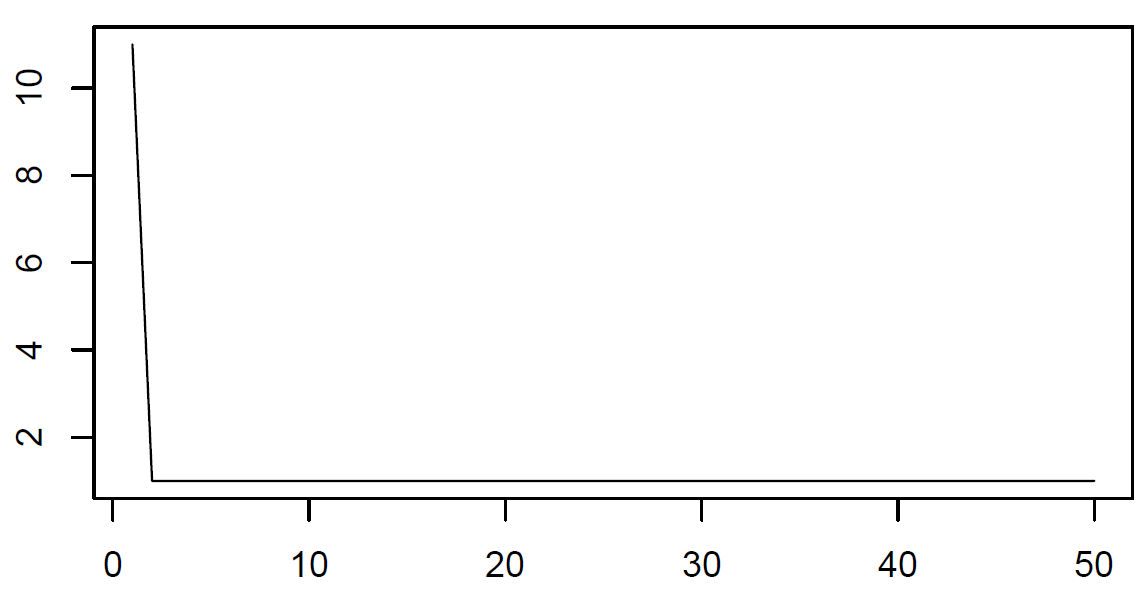
\includegraphics[, height = 2.2cm]{const_outl_graph_1.PNG}
%         \caption{График $\Re(\tX{X})$.}
%     \end{center}
% \end{figure}
\begin{figure}[H]
     \begin{center}
        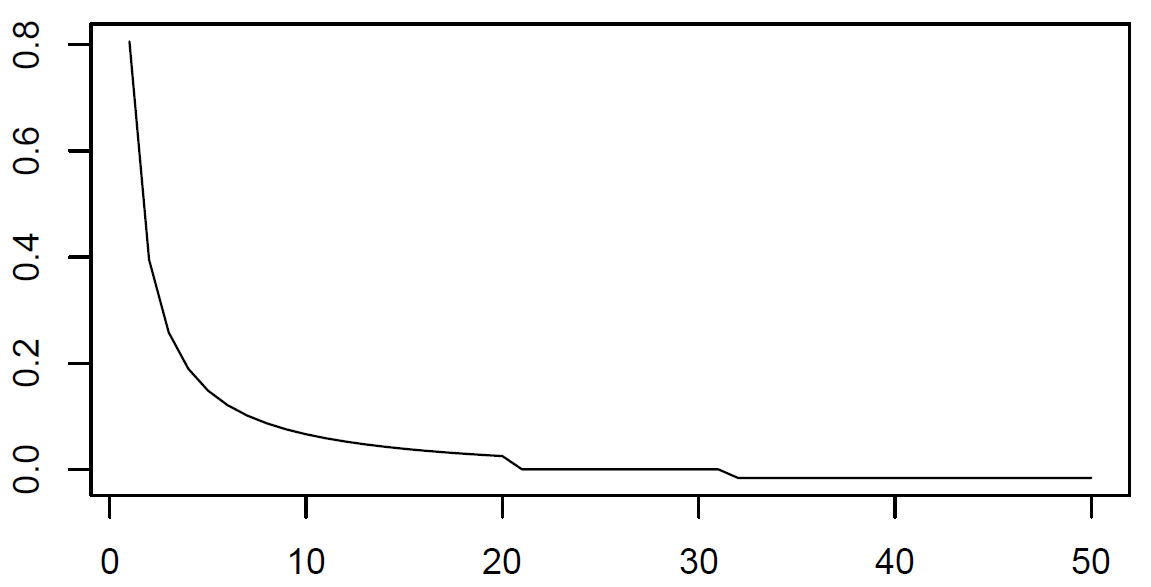
\includegraphics[, height = 5cm]{const_outl_err_1.PNG}
        \caption{График $\Re(\text{CSSA-}\tX{F}^{(1)})$.}
    \end{center}
\end{figure}
\footnote{Здесь хорошо бы добавить динамику по $k$, беря, скажем, $k = 1, 5, 10$.}
\end{frame}

\begin{frame}{Выброс: График первого порядка для $k = N / 2$}
Рассмотрим
$$s_l = 1 + \iu,$$
$\tX{R}$~--- выброс $10 + \iu 10$ на позиции $k = N / 2$, $N = 50$, $L = 20$.

% \begin{figure}[H]
%     \begin{center}
%         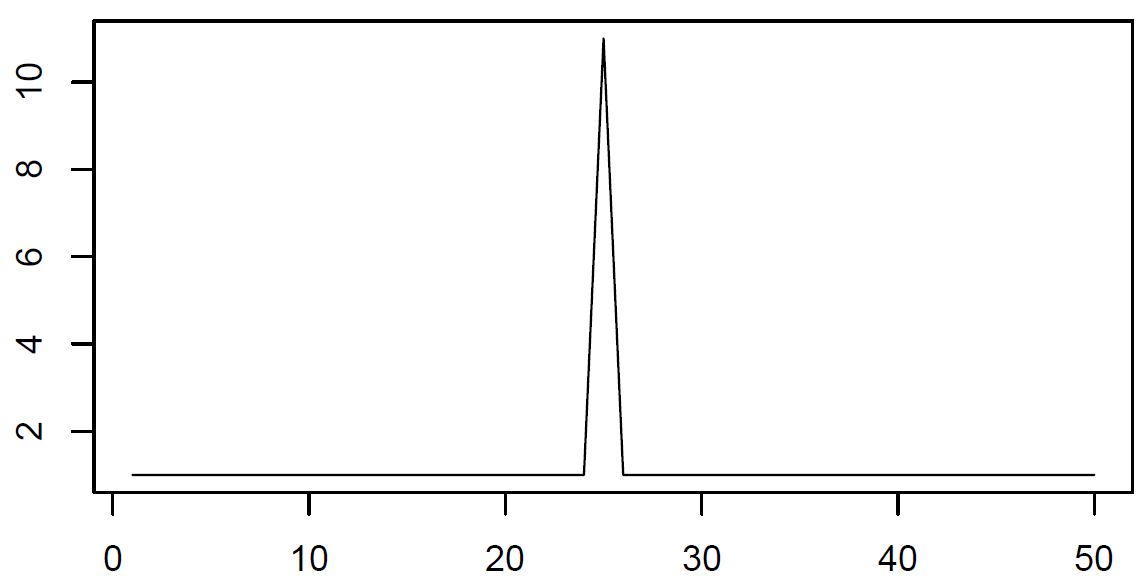
\includegraphics[, height = 2.2cm]{const_outl_graph_2.PNG}
%         \caption{График $\Re(\tX{X})$.}
%     \end{center}
% \end{figure}
\begin{figure}[H]
     \begin{center}
        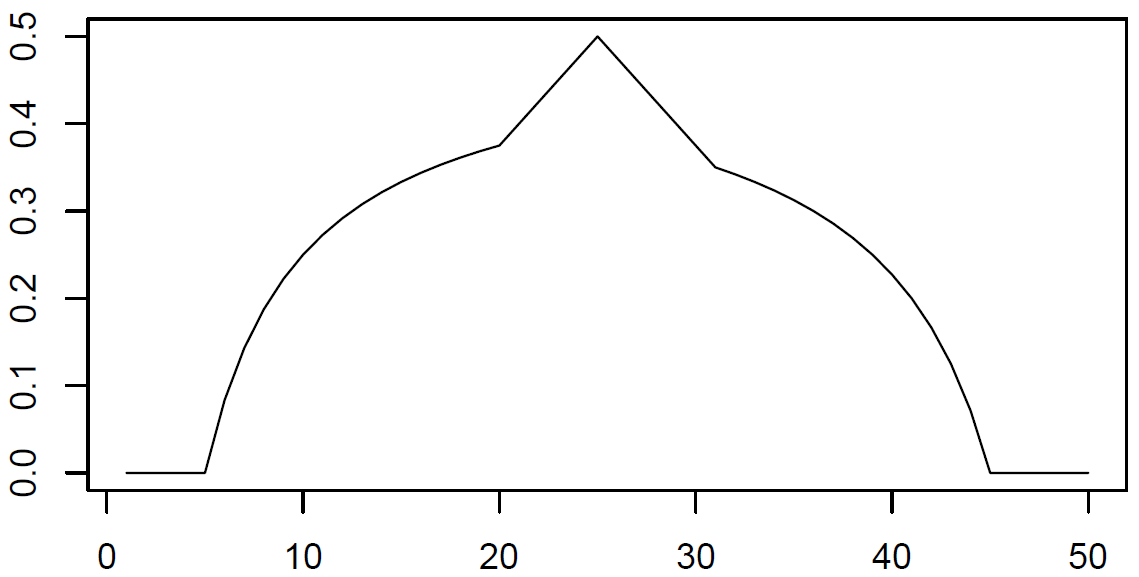
\includegraphics[, height = 5cm]{const_outl_err_2.PNG}
        \caption{График $\Re(\text{CSSA-}\tX{F}^{(1)})$.}
    \end{center}
\end{figure}
\footnote{Здесь хорошо бы добавить динамику по $L$, беря, скажем, $L = 5 (10?), 15 (20?), 25$.}
\end{frame}

\begin{frame}{Сравнение первого порядка и полной ошибок: Зашумлённые гармоники}
Рассмотрим
$$s_l = \cos(2 \pi l / 10) + \iu\cos(2 \pi l / 10 + \pi/4),$$
$\tX{R}$~--- белый шум с $\sigma^2 = 0.1$, $N = 9$, $L = 5$.
\begin{figure}[H]
	\begin{center}
		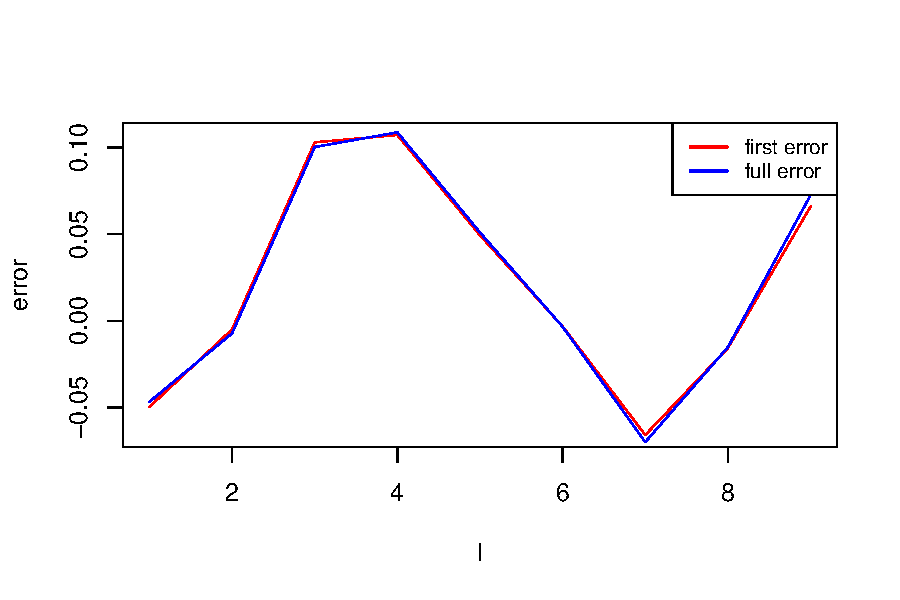
\includegraphics[width=0.6\linewidth]{img/first_vs_full_re.pdf}
		\caption{Вещественные части первого порядка и полной ошибок.}
		\label{fig:harm_noise}
	\end{center}
\end{figure}
\alert{Вывод:} Первый порядок почти совпадает с полной ошибкой.
\footnote{Нужно добавить шкалу по осям, хотя бы по Y}
\end{frame}

\begin{frame}{Сравнение первого порядка и полной ошибок: Константный сигнал с выбросом}

Рассмотрим
$$s_l = 1 + \iu,$$
$\tX{R}$~--- выброс $10 + \iu 10$ на позиции $k = L - 1$.

\begin{table}[H]
	\begin{center}
		\caption{Максимальное различие первого порядка и полной ошибок.}
		\label{tab:const_outl}
		\begin{tabular}{|c|c|c|c|c|}
			\hline
			$N$	& 50 & 100 & 400 & 1600 \\
			\hline
			$L = N / 2$ & 0.1313  & 0.0419  & 0.0033 & 0.0002 \\
			\hline
			$L = 20$ & 0.3074  & 0.1965  & 0.5655 & 0.6720 \\
			\hline
		\end{tabular}
	\end{center}
\end{table}

\alert{Вывод:} Первый порядок адекватно оценивает полную ошибку только в случае, когда $L$ и $K$ пропорциональны $N$.

\end{frame}

\begin{frame}{Заключение}
    \begin{itemize}
        \item Теория: при совпадении траекторных пространств комплексного ряда первые порядки ошибок для CSSA и SSA совпадают.
        \item Численные эксперименты: при случайном возмущении первый порядок адекватно описывает полную ошибку.
        \item $s_l = A\cos(2 \pi\omega l + \phi_1) + \iu B\cos(2 \pi\omega l + \phi_2)$, сдвиг не $\pi / 2$
        $$\mathbb{D}(\text{CSSA-}f^{(1)}_l) = \mathbb{D}(\text{SSA-}f^{(1)}_{\Re, l}) + \mathbb{D}(\text{SSA-}f^{(1)}_{\Im, l}).$$
        $s_l = Ae^{\pm \iu(2 \pi\omega l + \phi_1)}$
        $$\mathbb{D}(\text{CSSA-}f^{(1)}_l) \stackrel{?}{=} \frac{1}{2}[\mathbb{D}(\text{SSA-}f^{(1)}_{\Re, l}) + \mathbb{D}(\text{SSA-}f^{(1)}_{\Im, l})].$$
        \item Численные эксперименты: в случае выброса первый порядок адекватно оценивает полную ошибку при $L = \alpha N$ для больших $N$. При малых $L$ это не так.
        \item Теория: для $s_l = c_1 + \iu c_2$ с выбросом была получена аналитическая формула первого порядка. При $L = \alpha N$ ошибка стремится к $0$.
    \end{itemize}
\end{frame}


\end{document}
